\chapter{Data Preparation}

\begin{figure}[hbtp]
	\centering
	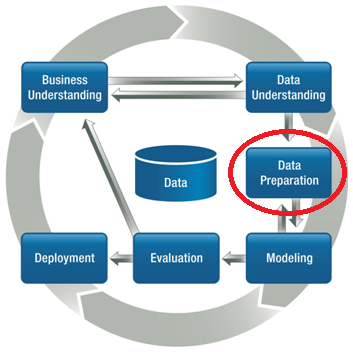
\includegraphics[width=0.5\textwidth]{./images/CRISPDM_3.png}
	\caption{CRISP-DM - Data Preparation}
	\label{CRISPDM_3}
\end{figure}

In questa fase si andranno a modellare i dati presenti nel dataset al fine di poter essere utilizzabili ai fini del processo del CRISP-DM.

\section{Criteri di Inclusione/Esclusione dei dati}

La totalità dei dati presenti nel dataset verrà utilizzata per il processo di KDD; non verrà fatta nessuna esclusione di istanza.

\section{Selezione dei dati}

\section{Campionamento}

Non verrà fatto nessun campionamento sui dati visto l'esiguo numero d istanze presenti, anzi si è deciso di utilizzare l'algoritmo \textit{SMOTE} al fine di migliorare il dataset... 

NAME
weka.filters.supervised.instance.SMOTE

SYNOPSIS
Resamples a dataset by applying the Synthetic Minority Oversampling TEchnique (SMOTE). The original dataset must fit entirely in memory. The amount of SMOTE and number of nearest neighbors may be specified. For more information, see 

Nitesh V. Chawla et. al. (2002). Synthetic Minority Over-sampling Technique. Journal of Artificial Intelligence Research. 16:321-357.

OPTIONS
classValue -- The index of the class value to which SMOTE should be applied. Use a value of 0 to auto-detect the non-empty minority class.

nearestNeighbors -- The number of nearest neighbors to use.

percentage -- The percentage of SMOTE instances to create.

randomSeed -- The seed used for random sampling.

\section{Feature Selection}

Per quanto riguarda la fase di feature selection, si è deciso di effettuare una selezione tra gli attributi presenti in quanto molti di questi risultano essere nulli nella maggior parte delle istanze presenti nel dataset, il che potrebbe, non solo non portare benefici al processo, ma potrebbe addirittura portare a rumore che causerebbe una errata predizione.
Come algoritmo scelto per effettuare la feature selection, si è utilizzato il \textit{CfsSubsetEval}, il quale valuta il "worth" del subset degli attributi considerando la singola correlazione di ognuno con l'attributo di classe. La ricerca nello spazio del subset degli attributi può essere realizzato essenzialmente attraverso la strategia best first la quale cerca \textbf{by greedy hillclimbing augmented with a backtracking facility.
La best first may start with the empty set of attributes and search forward, or start with the full set of attributes and search backward, or start at any point and search in both directions.}

By Weka:
Evaluates the worth of a subset of attributes by considering the individual predictive ability of each feature along with the degree of redundancy between them.
NAME
weka.attributeSelection.CfsSubsetEval

SYNOPSIS
CfsSubsetEval :

Evaluates the worth of a subset of attributes by considering the individual predictive ability of each feature along with the degree of redundancy between them.

Subsets of features that are highly correlated with the class while having low intercorrelation are preferred.

For more information see:

M. A. Hall (1998). Correlation-based Feature Subset Selection for Machine Learning. Hamilton, New Zealand.


By Wiki:
CFS Feature Set Evaluation

CFS is a correlation-based filter method CFS from [Hal98]. It gives high scores to subsets that include features
that are highly correlated to the class attribute but have low correlation to each other Let S be an attribute
subset that has k attributes, rcf models the correlation of the attributes to the class attribute, rff the
intercorrelation between attributes.


NAME
weka.attributeSelection.BestFirst

SYNOPSIS
BestFirst:

Searches the space of attribute subsets by greedy hillclimbing augmented with a backtracking facility. Setting the number of consecutive non-improving nodes allowed controls the level of backtracking done. Best first may start with the empty set of attributes and search forward, or start with the full set of attributes and search backward, or start at any point and search in both directions (by considering all possible single attribute additions and deletions at a given point).


OPTIONS
direction -- Set the direction of the search.

lookupCacheSize -- Set the maximum size of the lookup cache of evaluated subsets. This is expressed as a multiplier of the number of attributes in the data set. (default = 1).

searchTermination -- Set the amount of backtracking. Specify the number of 

startSet -- Set the start point for the search. This is specified as a comma seperated list off attribute indexes starting at 1. It can include ranges. Eg. 1,2,5-9,17.

\section{Data Cleaning}

\section{Construct Data}

\section{Integrate Data}
Non è stato necessario creare attributi derivati.

\section{Format Data}
Il dataset a disposizione era in formato .txt avente come delimitatore dei dati lo spazio e l'andata a capo come terminazione di una istanza. Questo ha reso necessario una conversione del dataset nel formato \textit{ARFF} in modo tale da poter essere utilizzato in Weka.
